\documentclass[11pt, handout]{beamer} % To remove reveals for printing.
%\documentclass[12pt]{beamer}


\usepackage{color}
\usefonttheme{professionalfonts} % using non standard fonts for beamer
\usefonttheme{serif} % default family is serif
%\usepackage{fontspec}
%\setmainfont{Liberation Serif}
\definecolor{blank}{gray}{1} %1 to hide



%\usetheme{CambridgeUS}

\newcommand{\bx}{\mbox{$\mathbf{x}$}}
\usepackage{amsfonts}           % let's be fancy:
\def\BE{\mathbb{E}}             % E(X) -- expectation
\def\BP{\mathbb{P}}             % P(X=1) -- probability
\usepackage{graphicx}           % import and rescale EPS figures
%\usepackage{pnas}
%\usepackage{showkeys}           %shows references
\usepackage{setspace, amsthm}
\usepackage{graphicx}
%\graphicspath{{./}{../Figures/} {../Graphs/} }

\graphicspath{{.}{Figures/}}

\usepackage{amsbsy,amssymb,amsmath, amsthm, psfrag}


\def\htheta{{\hat{\theta}}}
\newcommand{\bs}{\boldsymbol}
\newcommand{\ds}{\displaystyle}
\def\b{$\bullet $}
\def\ds{\displaystyle}
\def\BE{\mathbb{E}}
\def\Var{\mathbb{V}\mbox{ar}}
\def\cov{\mathbb{C}\mbox{ov}}
\def\cor{\mathbb{C}\mbox{or}}

\def\b{$\bullet $}
\def\ds{\displaystyle}
\def\BE{\mathbb{E}}
\def\Var{\mathbb{V}\mbox{ar}}
\newcommand{\re}{\mathrm{e}}
\newcommand{\rd}{\mathrm{d}}

\def\pgfb[#1][#2]{\pi(#1|#2)}
\def\vv{$^\wedge$}
\def\pgfa[#1][#2][#3][#4][#5][#6]{\pi(#1_{0:#2} #3|#4_{0:#5} #6)}

\def\pgf[#1][#2][#3][#4]{\pi(#1_{0:#2} |#3_{0:#4},\theta, \psi )}
%pgf for when we have x and z on separate sizes, with phi and theta in the conditional 
\def\xt {x_{0:t}}
\def\xtp{x_{0:t+1}}
\def\zt{z_{0:t}}
\def\ztp{z_{0:t+1}}

\def\rd {\mathrm{d}}


\addtolength{\topmargin}{0cm}  % decrease the margins
\addtolength{\textheight}{0cm}
\addtolength{\oddsidemargin}{0cm}
\setlength{\evensidemargin}{\oddsidemargin}
\addtolength{\textwidth}{0cm}

\def\ignore#1{{}}
\def\stnote#1{\textbf{\large #1}\marginpar{$\spadesuit$}}
\def\no{\noindent}
\def\etal{{\it et al. }}
\def\CD{\mathcal{D}}
\def\CN{\mathcal{N}}
\def\bm#1{{{\mbox{\boldmath $#1$}}}}  
\def\Var{\mathbb{V}\mbox{ar}}
\def\rd{\rm{d}}
   \newcommand{\eps}[1]{\(\epsilon_#1 \)}
\def\bias{\mbox{bias}}
\def\htheta{\hat{\theta}}
   
  \def\se{\mbox{se}} 
\def\hF{{\hat{F}}}
 \def\BI{\mathbb{I}}
 \def\Xi{X_{i}}
 \def\xi{x_{i}}
 
\newcommand{\e}{\varepsilon}
\newcommand{\al}{\alpha}
\newcommand{\s}{\sum_{i=1}^n}
\newcommand{\shat}{\hat{\sigma}^2}
\newcommand{\bhat}{\hat{\bbeta}}
\newcommand{\ahat}{\hat{\alpha}}
\newcommand{\be}{\mbox{\boldmath{$\varepsilon$}}\unboldmath}
\usepackage{bm}
%\newcommand{\bx}{\mbox{$\mathbf{x}$}}
\newcommand{\bz}{\mbox{$\mathbf{z}$}}
\newcommand{\xvec}{\mbox{$\bx_1,\ldots,\bx_n$}}
\newcommand{\yxvec}{\mbox{$y_1=\eta(\bx_1),\ldots,y_n=\eta(\bx_n)$}}
\newcommand{\by}{\mbox{$\mathbf{y}$}}
\newcommand{\boldm}{\mbox{$\mathbf{m}$}}
\newcommand{\bh}{\mbox{$\mathbf{h}$}}
\newcommand{\bt}{\mbox{$\mathbf{t}$}}
\newcommand{\bbeta}{\pmb{\beta}}
\newcommand{\bdelta}{\pmb{\delta}}
\newcommand{\btheta}{\pmb{\theta}}
\newcommand{\bo}[1]{\mbox{$\mathbf{#1}$}}
\newcommand{\yxpvec}{\mbox{$y_1'=\eta(\bx_1'),\ldots,y_{n'}'=\eta(\bx_{n'}')$}}
\newcommand{\xpvec}{\mbox{$\bx_1',\ldots,\bx_{n'}'$}}
\newcommand{\ri}{\mbox{$^{131}I$} }
\newcommand{\bX}{\bo{X}}
\newcommand{\bY}{\bo{Y}}
\newcommand{\betahat}{\mbox{$\hat{\bbeta}$}}
\newcommand{\sighat}{\mbox{$\hat{\sigma} ^2$}}

 \def\cor{\mbox{cor}}
   
\def\endexample{{\begin{flushright} $\square$ \end{flushright}}}

\setbeamertemplate{footline}[frame number]{}

%gets rid of bottom navigation symbols
\setbeamertemplate{navigation symbols}{}

%gets rid of footer
%will override 'frame number' instruction above
%comment out to revert to previous/default definitions
%\setbeamertemplate{footline}{}


\begin{document}

\frame{\frametitle{MAS472/6004: Computational Inference} 
\begin{center}
\Huge{ 
Chapter III\\
 Simulating random variables}
\end{center}


}



\frame {
 \frametitle{3.1 Generating Random Variables} \pause
\begin{itemize}
\item Inference techniques used so far have been based on
\textbf{simulation} \pause
\item We now consider how to simulate $X$
from $f_X(x)$.  \pause
\item In semester 1 used MCMC - but simpler methods needed in order
to do MCMC.  \pause
\item Starting point: generate $U$ from $U[0,1]$
distribution\pause \item Then consider transformation $g(U)$ to
obtain a random draw from $f_X(x)$.
\end{itemize}

How could we generate $U[0,1]$ r.v.s  with coin tosses?

}






\frame{

\frametitle{Sampling from $\bs{U(0,1)}$}

Need to simulate independent random variables uniformly distributed on $[0,1]$.

\medskip

{\bf  Definition:} A sequence of pseudo-random numbers $\{ u_i \}$ is a deterministic sequence of numbers in
$[0,1]$ having the same statistical properties as a similar sequence of random numbers. Ripley 1987.


\medskip

The sequence $\{ u_i \}$ is reproducible provided $u_1$ is known.

\medskip

A good sequence would be ``unpredictable to the uninitiated". 


}

\frame{

\frametitle{Congruential generators (D.H. Lehmer, 1949)}

The general form of a congruential generator is
\begin{align*}
N_i &= (aN_{i-1}+c) \text{ mod } M,\\
U_i &= N_i / M, ~\text{where integers}~ a, c \in [0,M-1]
\end{align*}
If $c=0$, it is called a {\em multiplicative congruential generator} (otherwise, {\em mixed}).


These numbers are restricted to the $M$ possible values
\[
0, ~~ \frac{1}{M}, ~~ \frac{2}{M}, ~~ \ldots , ~~ \frac{M-1}{M}.
\]
Clearly, they are {\em rational} numbers, but if $M$ is large they will 
 practically cover the reals in $[0,1]$.

 \medskip
 
 $N_1$: the \textbf{seed}. Can be re-set so you can reproduce same
set of uniform random numbers. In R, use \texttt{set.seed(i)}, where
$i$ an integer. 
}





\frame{

As soon as  some $N_i$ repeats, say,  $N_i=N_{i+T}$, then the whole subsequence repeats, i.e.
$N_{i+t}=N_{i+T+t}$, $t=1,2,\ldots$.

The least such $T$ is called the {\em period}.

A good generator will have a long period.

\medskip

The period cannot be longer than $M$ and also depends on $a$ and $c$.

Several useful Theorems exist concerning periods of congruential generators.
\medskip
For example, for $c>0$, $T=M$ if and only if 
\begin{enumerate}
\item $c$ and $M$ have no common factors (except 1),
\item $1=a$ (mod $p$) for every prime number that divides $M$, 
\item $1=a$ (mod $4$) if 4 divides $M$.
\end{enumerate}
}



\frame{

Usually $M$ is chosen to make the modulus operation efficient, and then $a$ and $c$ are chosen to make the period as long as possible. Ripley suggests $c=0$ or $c=1$ is usually a good choice.

\medskip

The NAG Fortran Library G05CAF
\[
M=2^{59} \qquad a=13^{13} \qquad c=0
\]
Another recommended one is
\[
M=2^{32} \qquad a=69069 \qquad c=1.
\]
so that
$$N_i=(69069N_{i-1}+1)\mbox{mod } 2^{32}$$
and
$$ U_i=2^{-32}N_i$$
}




\frame{\frametitle{Lattice structure}
Notice that for a congruential generator
$$N_i-aN_{i-1}=c-bM,$$
where $b>0$ is an integer. Therefore,
$$U_i-aU_{i-1}=\frac{c}{M}-b.$$
The LHS lies in $(-a,1)$ since $U_i\in [0,1)$.

Therefore, $b$ can take at most $a+1$ distinct values.

\medskip

If we plot points $(U_{i-1},U_i)$, all the points will lie on
at most $a+1$ parallel lines. }




\frame{
\begin{center}
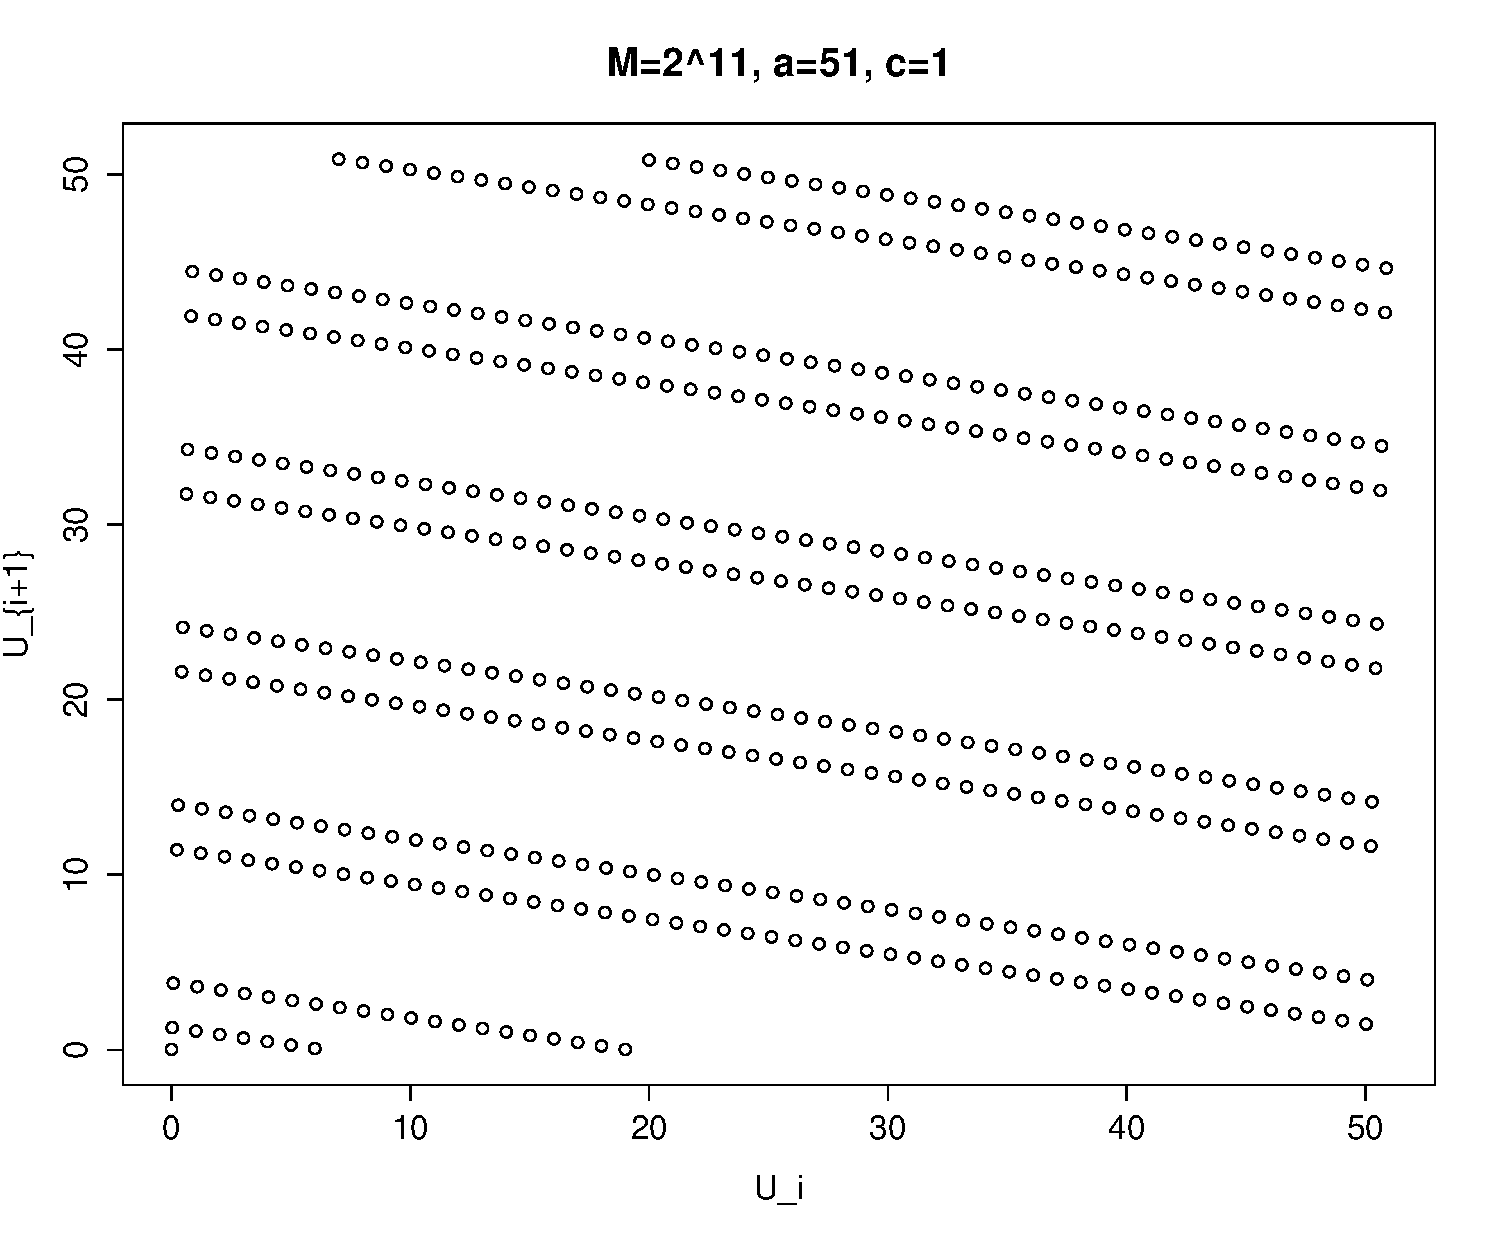
\includegraphics[scale=0.25]{cong_generator.pdf}
\end{center}

\vspace{-0.8cm}

All linear congruential generators exhibit this kind of lattice structure, not just for pairs  
$(U_{i-1},U_i)$, but also for triples $(U_{i-2},U_{i-1},U_{i})$, and in higher dimensions.

\medskip

A good generator is expected to have {\em fine lattice structure}, that is, 
points $(U_{i-k+1},\ldots,U_{i-1},U_{i})\in [0,1)^k$ must lie 
on many hyperplanes in $\mathbb{R}^k$ for all small $k$ ($k\ll M$). }




\frame{\frametitle{RANDU - lattice structure}
$M=2^{31}$, $a=2^{16}+3=65539$, and $c=0$. 
\medskip 

Once very popular, 
RANDU has eventually been found out to be a rather poor generator. 
\medskip

%\begin{align*}
%N_{i+2}&=(2^{16}+3)N_{i+1}+c_1 2^{31}\\
%&=(2^{16}+3)^2 N_i + c_2 2^{31} (2^{16}+3)+c_1 2^{31}\\
%&=(6 \times 2^{16}+9)N_i+2^{31} \{ \underset{c_3}
%{\underbrace{2^{16}c_2+3c_2+c_1+2N_i}} \}\\
%&=6(2^{16}+3)N_i-9N_i+c_3 2^{31}\\
%&=6N_{i+1}-9N_i + c_3 2^{31}\\
%\Longrightarrow&\quad N_{i+2}=6N_{i+1}-9N_i \mod 2^{31}.
%\end{align*}

}





\frame{\frametitle{RANDU - lattice structure II}
Let $U_i=N_i/m$ then for this generator
\[
U_{i+2}-6U_{i+1}+9U_i=k \text{ an integer}.
\]


Since $0 \leq U_i <1$
\[
-6 < U_{i+2}-6U_{i+1}+9U_i < 10.
\]
Therefore $k=-5,-4,\ldots,-1,0,+1,\ldots,9$.

Hence $k$ can take on 15 integer values only, and subsequently $(U_{i-2},U_{i-1},U_i)$ must lie 
on at most 15 parallel planes. 

\medskip 

This is an example of {\em coarse lattice structure}, unsatisfactory
coverage of $[0,1)^3$.



}

%%%%%%%%%%%%%%%%%%%%%%%%%%%%%%%%%%%%%%%%%%%%%%%%%%%%%%%%%%%%%%%%%%%%
%%%
%%% Non-uniform rvs
%%%
%%%%%%%%%%%%%%%%%%%%%%%%%%%%%%%%%%%%%%%%%%%%%%%%%%%%%%%%%%%%%%%%%%%%




\frame{
\frametitle{Generation from non-$U(0,1)$}

We have a sequence $U_1,U_2,U_3,\ldots$ of independent uniform random numbers in $[0,1]$.

\medskip

We want $X_1,X_2,\ldots$ distributed independently and identically from some specified distribution.

The answer is to transform the $U_1,U_2,\ldots$ sequence into $X_1,X_2,\ldots$ sequence.

The idea is to find a function $g(U_1,U_2,U_3,\ldots )$ that has the required distribution.

There are always many ways of doing this.  A good algorithm should be quick because millions of
random numbers may be required.

}






\frame{
\frametitle{3.2 The inversion method}

Let $X$ be any continuous random variable and define $Y=F_X (X)$, where $F_X$ is the distribution
function of $X$: $F_X(x)=P(X\leq x)$.  

{\bf Claim:} $Y \sim U[0,1]$.

{\bf Proof}
$Y\in [0,1]$ and the distribution function of $Y$ is
\begin{align*}
F_Y(y)&=P(Y \leq y)=P \big( F_X (X) \leq y \big)\\
&=P \big( X \leq F_X^{-1} (y) \big) = F_X \big( F_X^{-1} (y) \big) = y
\end{align*}
which is the distribution function of a uniform random variable on $[0,1]$.

\medskip


So whatever the distribution of $X$, $Y=F_X(X)$ is uniformly distributed on $[0,1]$.
The inversion method turns this backwards.  Let $U=F_X(X)$, then $X=F_X^{-1} (U)$.
\begin{itemize}
 \item 
So to generate $X\sim F_X$ take a single uniform variable $U$, and set $X=F_X^{-1} (U)$.

\end{itemize}



}


\frame{\frametitle{Example: exponential distribution}



Let $X\sim Exp(1/\lambda)$ (mean $\lambda$), i.e.
\[
f(x)=\lambda ^{-1} \re^{-x/\lambda} \quad (x\geq 0)
\]
\[
F(x)=\int_0^x \lambda^{-1} \re^{-z/\lambda} ~ \rd z = [-\re^{-z/\lambda}]_0^x=1-\re
^{-x/\lambda}.
\]
Set $U=1-\re^{-X/\lambda}$ and solve for $X$
\[
X=-\lambda \ln (1-U).
\]
Note that $1-U$ is uniformly distributed on $[0,1]$, so we might as well use
\[
X=-\lambda \ln U.
\]

{\bf 
Question:} What are the limitations of the inversion method?

} 











\frame{

\frametitle{Discrete distributions}

The inversion method works for discrete random variables in the following sense.

Let $X$ be discretely distributed with possible values $x_i$ having probabilities $p_i$.  So
\[
P(X=x_i)=p_i, \qquad \sum_{i=1}^k p_i=1.
\]
Then $F_X(x)=\sum\limits_{x_i \leq x} p_i$ is a step function.

Inversion gives $X=x_i$ if $\sum\limits _{x_j < x_i} p_j < U \leq \sum\limits _{x_j \leq x_i} p_j$
which clearly gives the right probability values.

\begin{itemize}
 \item Think of this as splitting $[0,1]$ into intervals of length $p_i$. The interval in which $U$ falls is the value of $X$.
\end{itemize}

{\bf Question:} What problems might we face using this method? Eg Consider a Poisson(100) distribuution.



}



\frame{\frametitle{Discrete distributions - example}


Let $X \sim \mathrm{Bin} (4,0.3)$.  The probabilities are
\[
P(X=0)=.2401, \quad P(X=1)=.4116, \quad P(X=2)=.2646
\]
\[
P(X=3)=.0756, \quad P(X=4)=.0081.
\]
\begin{align*}
\mbox{The algorithm says }&X=0 \quad \text{if} \quad 0 \leq U \leq .2401,\\
&X=1 \quad \text{if} \quad .2401 < U \leq .6517,\\
&X=2 \quad \text{if} \quad .6517 < U \leq .9163,\\
&X=3 \quad \text{if} \quad .9163 < U \leq .9919,\\
&X=4 \quad \text{if} \quad .9919 < U \leq 1.
\end{align*}
Carrying out the binomial algorithm means the following.  Let $U \sim U(0,1)$.
\begin{enumerate}
\item[1.]
Test $U \leq .2401$.  If true, return $X=0$.
\item[2.]
If false, test $U \leq .6517$.  If true, return $X=1$.
\item[3.]
If false, test $U \leq .9163$.  If true, return $X=2$.
\item[4.]
If false, test $U \leq .9919$.  If true, return $X=3$.
\item[5.]
If false, return $X=4$.
\end{enumerate}
}


\frame{\frametitle{Discrete distributions - example}
Consider the speed of this.  The expected number of steps (which roughly equates to speed) is
\[
1 \times .2401 + 2 \times .4116 + 3 \times .2646 + 4 \times .0756 + 4 \times .0081
\]
\[
=1+E(X)-0.0081=2.1919
\]

To speed things up we can rearrange the order so that the later steps are less likely.
\begin{enumerate}
\item[1.]
Test $U \leq .4116$.  If true return $X=1$.
\item[2.]
If false, test $U \leq .6762$.  If true return $X=2$.
\item[3.]
If false, test $U \leq .9163$.  If true return $X=0$.
\item[4.]
and 5. as before.
\end{enumerate}
Expected number of steps: $1 \times .4116 + 2 \times .2646 + 3 \times .2401 + 4 \times
(0.0956 + 0.0081)=1.9959$.  Approximate 10\% speed increase.


}




\frame{

\frametitle{3.3 Transformations}

\begin{enumerate}
\item[(a)]
If $U \sim U(0,1)$ set $V=(b-a)U+a$ then $V \sim U(a,b)$ where $a<b$.
\item[(b)]
If $Y_i$ are iid exponential with parameter $\lambda$ then
\[
X=\sum_{i=1}^n Y_i=-\frac{1}{\lambda} \sum_{i=1}^n \log U_i = -\frac{1}{\lambda} \log
\left( \prod_{i=1}^n U_i \right)
\]
has a $Ga(n,\lambda)$ distribution.
\item[(c)]
If $X_1 \sim Ga (p,1)$, $X_2 \sim Ga(q,1)$, $X_1$ and $X_2$ independent then
$Y=X_1 / (X_1 + X_2) \sim Be(p,q)$.

\item[(d)] Composition: if $$f=\sum_{i=1}^r p_i f_i$$ where $\sum p_i=1$ and each $f_i$ is a density, then we can sample from $f$ by first sampling $I$ from the discrete distribution $p=\{p_1, \ldots, p_r\}$ and then taking a sample from $f_I$.

\end{enumerate}

}




\frame{

\frametitle{The Box-M\"uller algorithm for the normal distribution}

We cannot generate a normal random variable by inversion, because $F_X$ is not known in closed
form (nor its inverse).




{\bf The Box--M\"uller method (1958)}.  Let $U_1,U_2 \sim U[0,1]$.  Calculate
\begin{align*}
X_1&=\sqrt{-2 \ln U_1} \cos (2 \pi U_2),\\
X_2&=\sqrt{-2 \ln U_1} \sin (2 \pi U_2).
\end{align*}
Then $X_1$ and $X_2$ are independent $N(0,1)$ variables.

The method is not particularly fast, but is easy to program and quite memorable.


}








\frame{\frametitle{3.4 Rejection Algorithm}
\begin{center}
\fbox{
\parbox{10cm}{
{\bf Fundamental Theorem of Simulation:}

Simulating $$X \sim f(x)$$ is equivalent to simulating

$$(X,U) \sim U\{(x,u): 0< u < f(x)\}.$$
}}
\end{center}

\medskip
Note that $f(x,u)=\mathbb{I}_{0<u<f(x)}$ so that
$$\int f(x,u) \rm{d} u= \int_0^{f(x)} \rm{d} u=f(x)$$
as required.

\medskip
Hence, $f$ is the marginal density of the joint distribution $(X,U) \sim U\{(x,u): 0< u < f(x)\}$.

}


\frame{\frametitle{Rejection  Algorithm Explained}
%{\small
The problem with this result is that simulating uniformly from the set 
$$ \{(x,u): 0< u < f(x)\}$$
may not be possible. 
A solution is to simulate the pair $(X,U)$ in a bigger set, where simulation is easier, and then take the pair if the constraint is satisfied.
%\vspace{-0.5cm}
\begin{center}
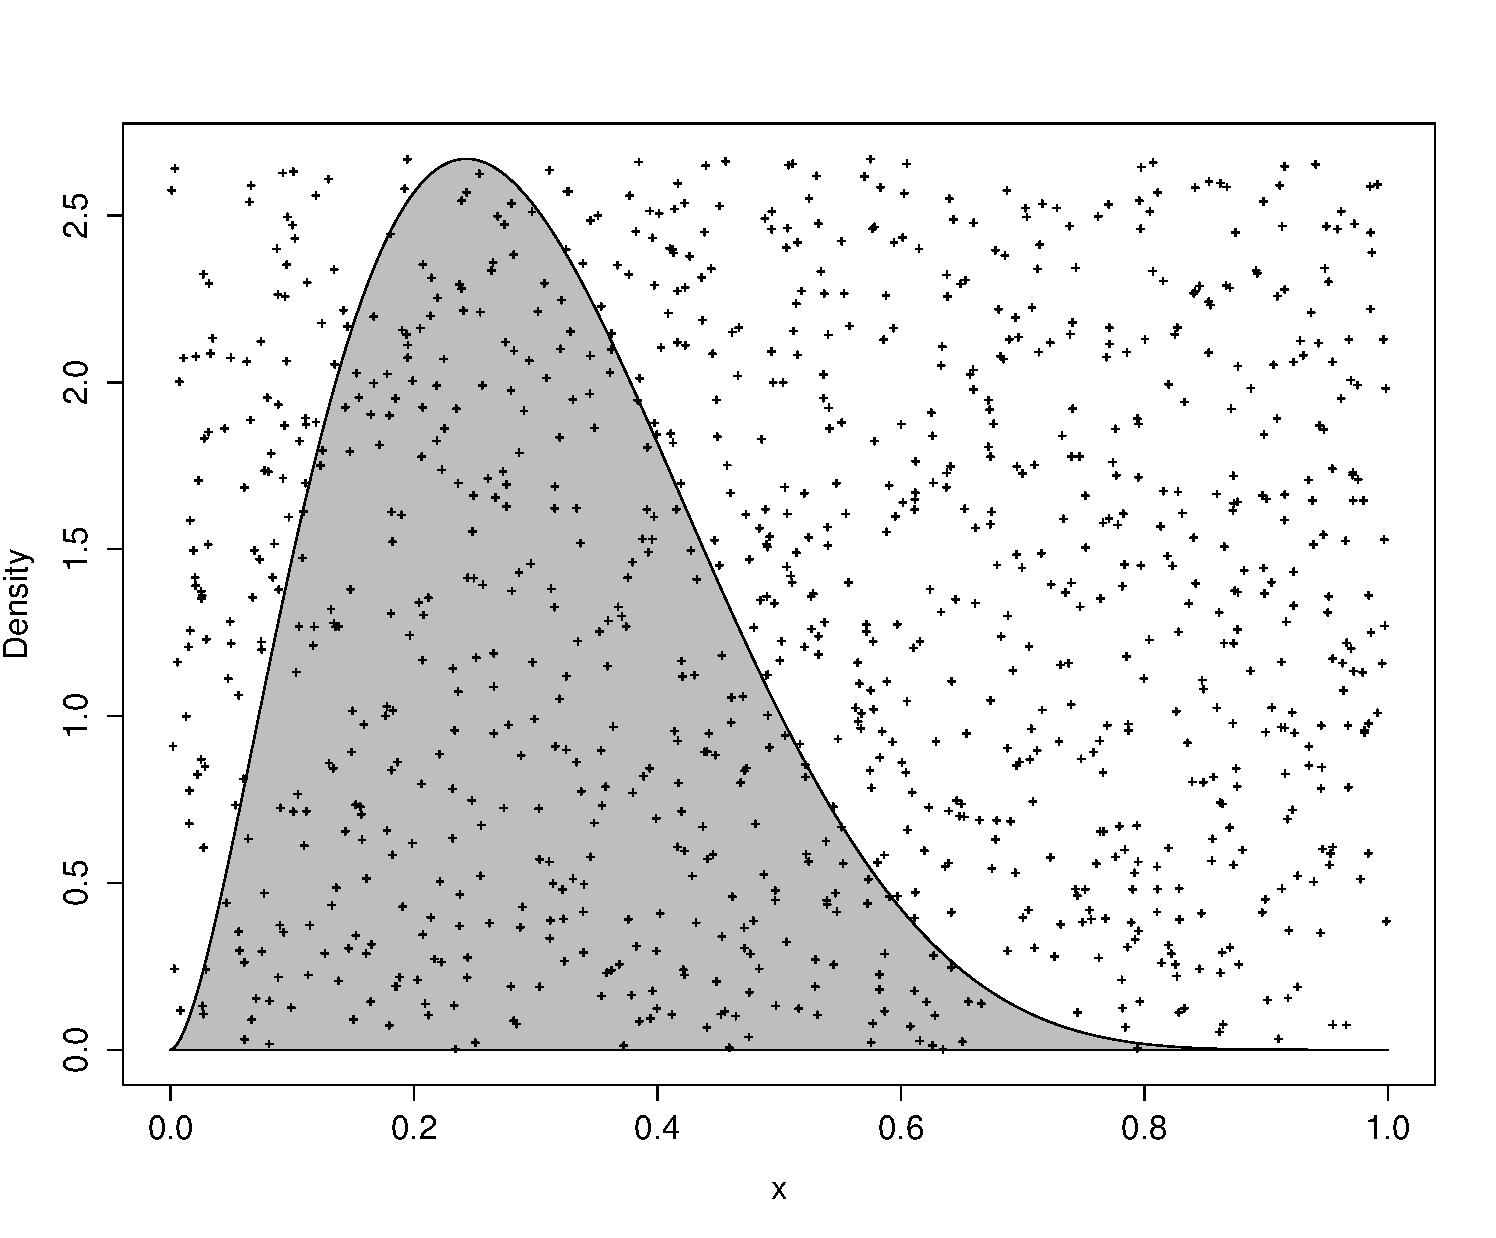
\includegraphics[scale=0.25]{rejectbox.pdf}
\end{center}

}


\frame{\frametitle{Rejection: Uniform bounding box}
Suppose that $f(x)$ is zero outside the interval $[a,b]$ (so that $\int_a^b f(x)\rm{d}x=1$) and that $f$ is bounded above by $m$. 
\begin{itemize}
 \item Simulate the pair $(Y,U) \sim U[a,b]\times[0,m]$ ($Y \sim U[a,b], \; U\sim U[0,m]$ independently). 
\item
Accept the pair  if the constraint $0<U <f(Y)$ is satisfied. 
\end{itemize}
This results in the correct distribution for the accepted $Y$ value, call it $X$.
\vspace{-0.5cm}
\begin{align*}
 \BP(X\leq x)&= \BP(Y\leq x| U<f(Y))\\
&= \frac{\int_a^x \int_0^{f(y)} \rm{d}u \rm{d} y}{\int_a^b \int_0^{f(y)} \rm{d}u \rm{d} y}\\
&=\int_a^x f(y) \rm{d} y.
\end{align*}

Note: we can use the rejection algorithm even if we only know $f$ upto a normalising constant (as is often the case in Bayesian statistics - see chapter 4).

}


\frame{\frametitle{Example: Sampling from a beta distribution}


Consider sampling from $X \sim \mathrm{Beta} (\alpha , \beta)$ for $\alpha,\beta>1$ which has pdf
\[
f(x)=\frac{\Gamma (\alpha+\beta)}{\Gamma (\alpha) \Gamma (\beta)} x^{\alpha-1}
(1-x)^{\beta-1} \quad 0<x<1.
\]
We note
\[
f(x) \propto f_1 (x)=x^{\alpha-1} (1-x)^{\beta-1} \quad 0<x<1
\]
and that 
$M=\underset{0<x<1}{\sup} x^{\alpha-1} (1-x)^{\beta-1}$
occurs at $x=\dfrac{\alpha-1}{\alpha+\beta-2}$ (mode) and hence
$$M=\frac{(\alpha-1)^{\alpha-1}(\beta-1)^{\beta-1}}
{(\alpha+\beta-2)^{\alpha+\beta-2}}.
$$

The rejection algorithm is
\begin{enumerate}
\item[1.]
Generate $Y \sim U(0,1)$ and $U \sim U(0,M)$.
\item[2.]
If $U \leq f_1(Y)=Y^{\alpha-1}(1-Y)^{\beta-1}$
then let $X=Y$ (accept) else go to 1 (reject).
\end{enumerate}



}



\frame{\frametitle{Generalising the Rejection Idea}

If the support of $f$ is not finite, then bounding it within a rectangle will not work.
Instead of using a box to bound the density $f(x)$ (ie requiring $f(x)<m$ for some constant $m$) we can use a function $m(x)$ such that $f(x)\leq m(x)$ for all $x$.

\medskip

Suppose the larger bounding set is
$$\mathcal{L} =\{(y,u) : 0<u<m(y)\}$$
then all we require is that simulation of a uniform from $\mathcal{L}$ is feasible. Note
\begin{itemize}
\item The closer $m$ is to $f$ the more efficient our algorithm.
\item Because $m(x)\geq f(x)$, $m$ cannot be a probability density. We write
$$m(x)=M g(x) \mbox{ where } \int m(x) \rm{d} x=\int M g(x) \rm{d} x = M$$
for some density $g$. 
\end{itemize}

}



\frame{\frametitle{Generalising the Rejection Idea II}
This suggests  a more general implementation of the fundamental theorem:
 \begin{center}
\fbox{
\parbox{10cm}{
{\bf Corollary:}
Let $X\sim f(x)$ and let $g(x)$ be a density function that satisfies $f(x)\leq Mg(x)$ for some constant $M\geq 1$. Then, to simulate $X \sim f$, it is sufficient to generate
$$Y \sim g \qquad \mbox{ and }\qquad U|Y=y \sim U(0, Mg(y))$$ 
and set $X=Y$ if $U\leq f(Y)$.
}}
\end{center}

{\bf Proof:}
\begin{align*}
 \BP(X\in A)&=\BP(Y \in A| U\leq f(Y))\\
&=\frac{\int_A \int_0^{f(y)} \frac{\rm{d}u}{Mg(y)}g(y) \rm{d} y}{\int \int_0^{f(y)} \frac{\rm{d}u}{Mg(y)}g(y) \rm{d} y}\\
&= \int_A f(y) \rm{d}y
\end{align*}
}




\frame{

\frametitle{The Rejection Algorithm}

The rejection algorithm is usually stated in a slightly modified form:

 \begin{center}
\fbox{
\parbox{10cm}{
\begin{enumerate}
\item[] {\bf Rejection Algorithm}

\item[] If $g$ is such that $f/g$ is bounded, so there exists  $M$ such that $Mg(x) \geq f(x)$ for all $x$ then
\item[1.]
Generate $Y$ from density $g$, and $U$ from $U(0,1)$.
\item[2.]
If $U \leq f(Y) / Mg(Y)$ set $X=Y$.  Otherwise, return to step 1.
\item[] produces simulations from $f$

\end{enumerate}
}}
\end{center}
\medskip

We keep sampling new $Y$ and $U$ until the condition is satisfied.

\medskip

Exercise: Convince yourself that these two descriptions of the rejection algorithm are the same.
}


\frame{\frametitle{Example: Sampling from a beta distribution revisited}


Use rejection to sample from $X \sim \mathrm{Beta} (\alpha,\beta)$.
Let $g(y)=\alpha y^{\alpha-1}$, $0<y<1$, then
\[
\frac{f_1(x)}{g(x)}=\frac{(1-x)^{\beta-1}}{\alpha}
\quad \text{is bounded if and only if } \beta \geq 1
\]
Then $\ds{
M=\sup_x \left\{ \frac{f_1(x)}{g(x)}\right\} =\frac{1}{\alpha}}$ occurs at $x=0$.

\begin{enumerate}
\item[1.]
Simulate $Y$ with pdf $g(y)=\alpha y^{\alpha-1}$, $0 < y < 1$ and $U \sim U(0,1)$.
\item[2.]
If $U \leq \dfrac{f_1(Y)}{Mg(Y)}=\dfrac{(1-Y)^{\beta-1}}{\left( \frac{1}{\alpha}\right) \alpha}
=(1-Y)^{\beta-1}$ then set $X=Y$ else go to 1.
\end{enumerate}


}

\frame{

How to simulate $Y$ with pdf $g(y)=\alpha y^{\alpha-1}$?
\begin{itemize}
 \item 
We note that the cdf of $Y$ is $G(y)=y^\alpha$, $0<y<1$.

\item
Therefore we can use inversion. Let $Z \sim U(0,1)$ then solve $Z=G(Y)=Y^\alpha$ and so $Y=Z^{\frac{1}{\alpha}}$.
\end{itemize}



\textbf{Full algorithm is}:
\begin{enumerate}
\item[1.]
Generate $U \sim U(0,1)$ and $Z \sim U(0,1)$.  Let $Y=Z^{\frac{1}{\alpha}}$.
\item[2.]
If $U \leq (1-Y)^{\beta-1}$ then set $X=Y$ else go to 1.
\end{enumerate}

\begin{center}
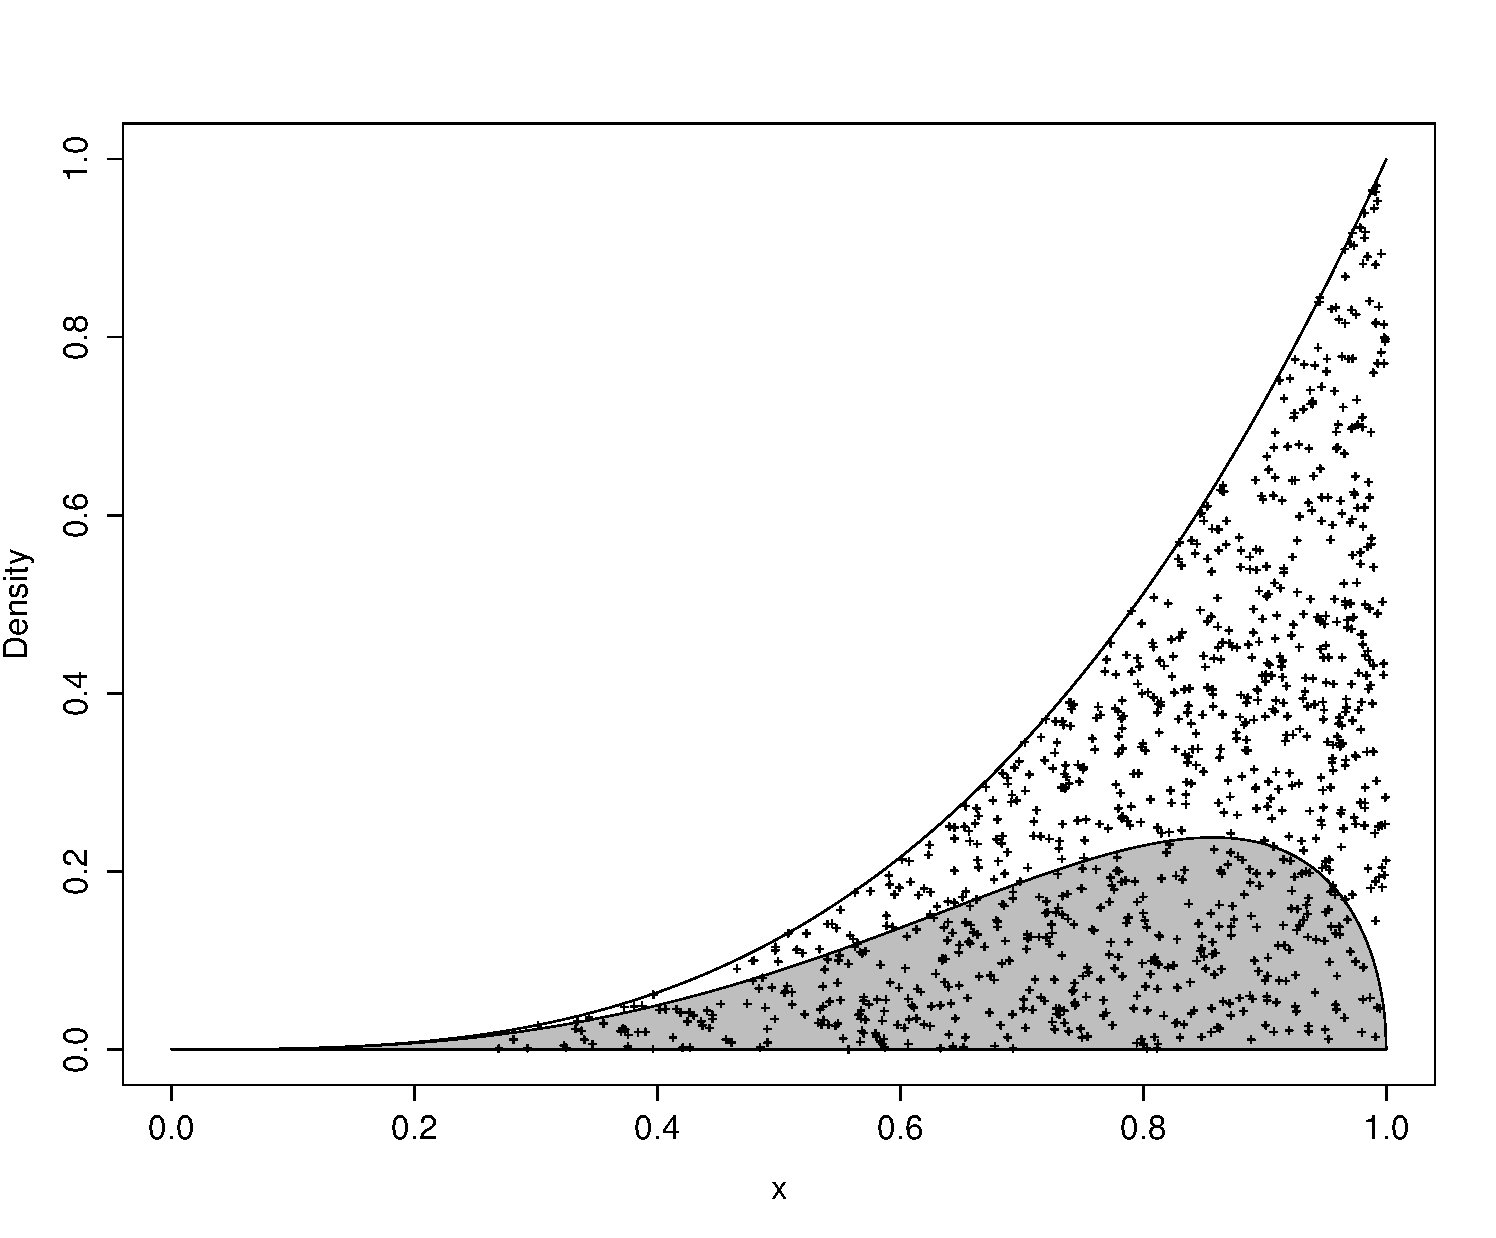
\includegraphics[scale=0.25]{rejectbeta.pdf}
\end{center}
}



\frame{

\frametitle{Efficiency of the rejection method}
{\small
Each time we generate a $(Y,U)$ pair,
\[
\text{Prob(Reject)}=
P\big( U \geq f(Y) / Mg(Y) \big) = 1-\frac{1}{M}, \quad
\text{Prob(Accept)}=\frac{1}{M}.
\]
The number of tries until we accept $Y$ is a geometric random variable 
with expectation $M$.

\medskip

Note that $M$ here must be calculated with the normalised density $f$, i.e., $M = \sup \frac{f(x)}{g(x)}$.

If we used an unnormalised density $f_1(x)$, where $\int f_1(x) {\rm d} x = c$, so that $f(x)=\frac{1}{c}f_1(x)$, then if we used
$$M = \sup \frac{f_1(x)}{g(x)}$$
the acceptance rate is
$$\BP(\mbox{Accept}) = \frac{c}{M}$$
}}


\frame{
For maximum efficiency, we want $M$ as small as possible, i.e.\ $\sup f(x)/g(x)$ as
small as possible.  This means finding a $g$ that 
\begin{enumerate}[(a)] 
\item we can sample from efficiently, and 
\item mimics $f$ as closely as possible.  
\end{enumerate}
There are many good generators based on rejection from a
well-chosen $g$.

}







\frame{\frametitle{Rejection Example III}


Let $\theta$ have von Mises distribution with pdf
\[
f(\theta)=\frac{\exp(k \cos \theta)}{2 \pi I(k)} \quad 0< \theta < 2 \pi \quad (k\geq 0)
\]
where $I(k)$ is the normalising constant.

Let $f_1(\theta)=\dfrac{1}{2 \pi} \exp (k \cos \theta)$, $0<\theta < 2 \pi$.

$Y \sim U(0,2 \pi)$ so that $g(y)=\dfrac{1}{2 \pi}$, $0 < y < 2 \pi$.

Then
\[
M = \sup_{\theta} \left\{ \frac{f_1(\theta)}{g(\theta)} \right\} =\sup_{\theta}
\{ \exp (k \cos \theta) \} =\exp k.
\]
Let $U \sim U(0,1)$.

If
\[
U \leq \frac{f_1(Y)}{Mg(Y)}=\frac{\exp (k \cos Y)}{2 \pi \cdot \dfrac{1}{2 \pi} \cdot \exp k}
=\exp \big( k (\cos Y-1) \big)
\]
we accept $\theta=Y$ otherwise reject.


}


%
%\frame{
%
%\frametitle{Improving efficiency}
%
%Another factor in the speed of rejection algorithms is the need to calculate $f(y)/g(y)$ every
%time when in fact $f$ is often a rather complex function and therefore expensive or difficult to
%calculate.
%
%Suppose, however, we can find two more functions $h_1(x)$ and $h_2(x)$, which are quick to
%calculate and such that
%\[
%h_1(x) \leq \frac{f(x)}{Mg(x)} \leq h_2 (x) \quad \text{for all } x.
%\]
%Quick acceptance if $U \leq h_1 (Y)$.\newline
%Quick rejection if $U \geq h_2 (Y)$.
%
%}
%
%\frame{

%%\frametitle{`Squeezing'}
%%
%%The squeeze rejection algorithm:
%%\begin{enumerate}
%%\item[1.]
%%Generate $Y$ from $g$ and $U$ from $U(0,1)$.
%%\item[2.]
%%If $U \leq h_1 (Y)$, return $X=Y$.
%%\item[3.]
%%Otherwise, if $U \geq h_2 (Y)$, reject $Y$ and go to step 1.
%%\item[4.]
%%Otherwise, if $U \leq \dfrac{f(Y)}{Mg(Y)}$, return $X=Y$.
%%\item[5.]
%%Otherwise, go to step 1.
%%\end{enumerate}
%%If the squeeze functions $h_1$ and $h_2$ are well chosen, we will rarely actually need to calculate
%%$f/g$.  If $g$ is well chosen in the first place, $f(x)/Mg(x)$ will be close to one for most $x$, and
%%so the upper squeeze function $h_2$ will make only a minor improvement, but $h_1$ can make a
%%big difference.
%%
%%}
%%
%%
%%
%%\frame{\frametitle{Example of `Squeezing' I}
%%
%%Suppose we wish to generate $X \sim N(0,1)$ using rejection from Cauchy random variable with pdf
%%\[
%%g(y)=\frac{1}{\pi(1+y^2)}\quad -\infty < y < \infty .
%%\]
%%\begin{equation*}
%%\mbox{Let } M=\sup_y \left\{ \frac{f(y)}{g(y)} \right\}=\sup_y \left\{ \frac{\frac{1}{\sqrt{2\pi}} \exp
%%\{-y^2 / 2\}}{\frac{1}{\pi(1+y^2)}} \right\}=\sqrt{\frac{2\pi}{e}} 
%%\end{equation*}
%%which occurs at $y=\pm 1$.
%%Acceptance condition for the rejection method is
%%\[
%%U \leq \frac{f(Y)}{Mg(Y)}=\frac{\sqrt e}{2} (1+Y^2)e^{-Y^2/2}.
%%\]
%%The expression on the right hand side may be considered to be complicated/expensive to compute.
%%
%%We
%%note $\exp \left\{ -\dfrac{Y^2}{2} \right\} \geq 1-\dfrac{Y^2}{2}$ hence lower squeeze test is
%%\vspace{-0.4cm}
%%\[
%%U \leq \frac{\sqrt e}{2} (1+Y^2) \left( 1-\frac{Y^2}{2} \right) .
%%\]
%%
%%}
%%
%
%\frame{\frametitle{Example of `Squeezing' II}
%
%Consider sampling from an exponential on $(0,2)$ such that the pdf of $X$ is
%\[
%f(x)=\frac{\re^{-x}}{1-\re^{-2}} \quad 0<x<2.
%\]
%Let $f_1(x)=\re^{-x}$, $0<x<2$,
%
%and $g(y)=\frac{1}{2}$, $0<y<2$, so that $Y \sim U(0,2)$.
%
%Let $\ds{
%M=\sup_x \left\{ \frac{f_1(x)}{g(x)} \right\}=\sup_x 2 \re^{-x}=2}$.
%
%If $U \leq \dfrac{f_1(Y)}{Mg(Y)}=\re^{-Y}$ then accept $X=Y$.
%
%}
%\frame{\frametitle{Example of `Squeezing' II -ctd}
%
%Apply squeezing to $U \leq \re^{-Y}$.
%
%Notice $\re^x \geq 1+x$ for all $x$, therefore
%\[
%1-x \leq \re^{-x} \leq \frac{1}{1+x}.
%\]
%This is true for `$x$' $=x-a$, hence $\re^{-a}(a+1-x) \leq \re^{-x} \leq
%\dfrac{\re^{-a}}{1-a+x}$.
%
%Therefore set $h_1(x)=\re^{-a}(a+1-x)$ and $h_2(x)=\re^{-b} / (1-b+x)$.
%
%The full algorithm is
%\begin{enumerate}
%\item[1.]
%Sample $Y \sim U(0,2)$, $U \sim U(0,1)$.
%\item[2.]
%If $U \leq \re^{-a}(a+1-Y)$ go to 5.
%\item[3.]
%If $U> \re^{-b}/(1-b+Y)$ go to 1.
%\item[4.]
%If $U > \re^{-Y}$ go to 1.
%\item[5.]
%Return $X=Y$.
%\end{enumerate}
%$a$ and $b$ may be chosen to maximize probability of acceptance
%in which case it can be shown that $a=1$ and $b=.662$.
%}
%
%
%

\frame{

\frametitle{Truncated distributions} \pause Suppose we wish to
sample $X$ from the following distribution:
\begin{equation*}
f_X(x)\propto \left\{\begin{array}{cc} g_X(x) & \mbox{for } x \in A
\\ 0 & \mbox{otherwise} \end{array} \right.
\end{equation*}
 \pause where $g_X(x)$ is a known density that we can sample from, e.g.
$g_X(x)$ is the $N(0,1)$ density, and $A=[0,\infty)$. \pause
\begin{equation*}
f_X(x)= \left\{\begin{array}{cc} k\,g_X(x) & \mbox{for } x \in A
\\ 0 & \mbox{otherwise} \end{array} \right. \end{equation*}
 \pause where $k$ is a normalising constant, given by \begin{equation*}
k^{-1}= \int_A g_X(x)dx
\end{equation*}}

\frame{
\begin{equation*}
f_X(x)\propto \left\{\begin{array}{cc} g_X(x) & \mbox{for } x \in A
\\ 0 & \mbox{otherwise} \end{array} \right.
\end{equation*}

 \pause Consider using rejection method to sample $X$ from $f_X(x)$.
We sample $Y$ from the full (non-truncated) density $g_X(x)$.
\begin{equation*}
\frac{f_X(x)}{g_X(x)}=\left\{\begin{array}{cc} k & \mbox{if } x\in A
\\ 0 &\mbox{otherwise}\end{array} \right.
\end{equation*}

}

\frame{

So $M=\mbox{sup}_x \frac{f_X(x)}{g_X(x)}=k$. \pause \\ Rejection
algorithm: sample $u$ from $U[0,1]$ and $y$ from $g_Y(y)$, and
accept $X=y$ if $u\le \frac{f_X(y)}{M\,g_Y(y)}$. \pause \\ But since
\begin{equation*}
\frac{f_X(x)}{M\,g_X(x)}=\left\{\begin{array}{cc}
\frac{f_X(x)}{k\,g_X(x)} = 1 & \mbox{if } x\in A \\ 0
&\mbox{otherwise}\end{array} \right.
\end{equation*}
 \pause we will always have $u\le \frac{f_X(y)}{M\,g_Y(y)}$ if $y\in A$ ,
and $u\ge \frac{f_X(y)}{M\,g_Y(y)}$ if $y \notin A$.\\ \pause  So we
don't need to sample $u$.  \pause 
Can just do
\begin{enumerate}\item generate $y$ from $g_Y(y)$ \pause \item if $y\in A$, accept $X=y$ \pause 
\item otherwise, return to step 1.  \pause 
\end{enumerate}
 As usual, acceptance
probability will be high if $M$ is small, i.e $\int_A g_Y(y)\, dy$
is near 1. So if the truncated region is large, rejection sampling
will be inefficient.


 }





\frame{

\frametitle{3.5 Multivariate generators}

Now suppose we want to generate a random vector $\bs{X}=(X_1,\ldots,X_p)$ from density
$f(\bs{x})$.  We can note the following simple points.
\begin{enumerate}
\item[1.]
If the elements of $\bs{X}$ are to be independent, i.e.
\[
f(\bs{x})=f_1(x_1)f_2(x_2) \ldots f_p(x_p),
\]
then we can separately generate $X_1$ from $f_1$, $X_2$ from $f_2, \ldots , X_p$ from $f_p$
using different uniforms.
\item[2.]
Inversion no longer works as the theorem can't be generalised.
\item[3.]
Rejection \textit{does} work.  If we can generate from $g(\bs{x})$ (and $g$ may be a product
of independent components) and find $\ds{M\geq \sup_{\bs{x}} \frac{f(\bs{x})}{g(\bs{x})}}$ and
otherwise reject.
\end{enumerate}

}\frame{

\frametitle{Sequential methods}

We can obviously write
\[
f(\bs{x})=f_1(x_1) f_2(x_2 | x_1) f_3 (x_3 | x_1,x_2) \ldots \, .
\]
So we can first generate $X_1$ from $f_1$.  Then for that given value of $X_1$, generate $X_2$
from $f_2$, and so on.


}



\frame{ \frametitle{Example}

REPLACE THIS EXAMPLE WITH Normal inverse gamma instead.

We wish to sample $\{\theta,\phi\}$ from the density function
\begin{equation*}
f(\theta,\phi)\propto
\phi^3\exp\{-1(1+5\phi)\theta^2+40\phi\theta-81\phi\}.
\end{equation*}
 \pause Firstly, it can be shown that the marginal density of $\phi$ is
\begin{equation*}
f(\phi)\propto
\phi^3(1+5\phi)^{-1/3}\exp\left\{-\phi\left(1+\frac{80}{1+5\phi}\right)\right\}.
\end{equation*}

}

\frame{

Additionally, the conditional distribution of $\theta|\phi$ is
normal:
\begin{equation*}
\theta|\phi \sim
N\left(\frac{20\phi}{1+5\phi},\frac{1}{2(1+5\phi)}\right).
\end{equation*}

\pause

To sample from $f(\theta,\phi)$ we could first sample $\phi$ from
$f(\phi)$, using rejection sampling, then generate $Z$ from
$N(0,1)$, and finally set
\begin{equation*}
\theta=\frac{20\phi}{1+5\phi}+\frac{1}{\sqrt{2(1+5\phi)}}Z.
\end{equation*}

\pause

\textbf{ Multivariate normal distributions}\\
Consider generating $\bX$ from $N(\bo{m},V), $ for some non-diagonal
matrix $V$, given a sample of independent standard normal random
variables $Z_1,Z_2,\ldots$.
\\ \pause

One technique involves the use of the \textbf{Cholesky square root}
of the matrix $V$. For any (symmetric, square) positive definite
matrix $V$, we can find a square root $U$, such that $ U^TU=V. $

}

\frame{

 Multiple solutions for $U$, but upper triangular matrix $U$ known
as the Cholesky square root. To find the Cholesky square root of a
matrix $V$ in R, type \texttt{chol(V)}.\\ \pause Define $\bo{Z}\sim
N(\bo{0},I)$ (equal dimension to $\bX$), consider
$\bo{Y}=\bo{m}+U^T\bo{Z}$. Then have $\bo{Y}$ normally distributed,
(each element of $\bo{Y}$ is linear combination of the elements of
$\bo{Z}$),\pause and
\begin{eqnarray*}
E(\bo{m}+U^T\bo{Z})&=&\bo{m},\\
Var(\bo{m}+U^T\bo{Z})&=&U^TIU=V,
\end{eqnarray*}
(with $I$ the identity matrix, the variance of $\bo{Z}$).\\ \pause
Hence to generate $\bo{X}$, we generate independent standard normal
random variables $\bo{Z}$, and then transform them by
$\bo{m}+U^T\bo{Z}$ to obtain $\bo{X}$.

}




%\frame{Next year, add more on IS. Concept of a weighted sample $\{\theta_i, p_i\}$, how to use this to estimate means, quantiles etc. Look at Robert's Monte Carlo with R book.}

\frame{

\frametitle{3.6 Importance sampling}

In order to estimate an integral of the form $\int h(x) f(x)\rd x$ we find that it is sometimes better to generate  values not from the distribution $f(x)$, but instead from some other distribution $g(x)$ and to then account for this by using a weighting. This is the idea behind importance sampling. To introduce the idea we consider a simple example.


}

\frame{\frametitle{Example of Monte Carlo/Importance Sampling}


Let $X$ be Cauchy $f(x)=\dfrac{1}{\pi (1+x^2)}$, $-\infty <x< \infty$.

Let $\ds{\theta=P(X>2)=I=\int_2^\infty \frac{1}{\pi(1+x^2)}~\rd x}$ ($=0.1476$).

Use Monte Carlo Methods to estimate $\theta$.

\begin{enumerate}
\item[(i)]
Generate $n$ Cauchy variates, $X_1, \ldots, X_n$.

Let $Y_1$ be the number that are greater than 2, $Y_1=\sum\mathbb{I}_{X_i>2}$. Then $Y_1 \sim B(n,\theta)$ so that
\[
E(Y_1)=n\theta , \quad V(Y_1)=n \theta (1-\theta)
\]
\[
\hat{\theta}_1 = \frac{Y_1}{n}
\]
\[
E(\hat{\theta}_1)=\frac{E(Y_1)}{n}=\frac{n\theta}{n}=\theta
\]
and
\[
V(\hat{\theta}_1)=\frac{V(Y_1)}{n^2}=\frac{n\theta(1-\theta)}{n^2}=
\frac{\theta(1-\theta)}{n}=\frac{0.126}{n}.
\]
\end{enumerate}



}





\frame{\frametitle{Example of Monte Carlo/Importance Sampling - II}

\begin{enumerate}

\item[(ii)]
Note that $\theta=\frac{1}{2} P(|X|>2)$ - we want to use this to reduce the variance of our estimator $\hat{\theta}$.

Generate $n$ Cauchy variates.

Let $Y_2$ be the number that are greater than 2 in modulus

then $Y_2 \sim B(n,2\theta)$

and $\hat{\theta}_2=\frac{1}{2} \dfrac{Y_2}{n}$
\[
\Longrightarrow E(\hat{\theta}_2)=\tfrac{1}{2} \frac{E(Y_2)}{n}=\tfrac{1}{2} \cdot
\frac{n2\theta}{n}=\theta
\]
and
\[
V(\hat{\theta}_2)=\frac{V(Y_2)}{2^2 n^2}=\frac{n2\theta(1-2\theta)}{2^2 n^2}=
\frac{\theta(1-2\theta)}{2n}=\frac{0.052}{n}.
\]

\end{enumerate}
}



\frame{\frametitle{Example of Monte Carlo/Importance Sampling - III}

\begin{enumerate}
\item[(iii)] 

The relative inefficiency of these methods is due to generation of values outside the domain of interest $[2, \infty)$.

Alternatively note we can write
\[
\theta =  \frac{1}{2} - \int_0^2 \frac{1}{\pi(1+x^2)}~\rd x.
\]
This integral can be considered the expectation of $h(X)=\frac{2}{\pi(1+x^2)}$ where $X \sim U[0,2]$ as the density of $U[0,2]$ is $ g(x)=1/2$.

An alternative method of evaluation of $\theta$ is therefore
$$\hat{\theta}_3=\frac{1}{2} -\frac{1}{n} \sum_{i=1}^n h(U_i)$$
where $U_i \sim U[0,2]$.
\end{enumerate}
}

\frame{\frametitle{Example of Monte Carlo/Importance Sampling - IV}
We can see that 
$$\BE(\hat{\theta}_3)=\frac{1}{2}-\frac{1}{n} \sum_{i=1}^n \int_0^2 \frac{2}{\pi(1+x^2)}\rd x    =\frac{1}{2}-\BP(0<X<2)$$
where $X\sim$ Cauchy, so that it too is an unbiased estimator.

\medskip
The variance of $\hat{\theta}_3$ is $\Var(h(U))/n$ and we can see that
\begin{align*}
 \BE h(U) &= \int_0^2 h(x)\frac{1}{2}\rd x=0.5-0.1475=0.3525\\
\BE h(U)^2&=\int_0^2 h(x)^2 \frac{1}{2} \rd x= \int_0^2 \frac{2}{\pi^2(1+x^2)^2} \rd x\\
&=\frac{1}{\pi^2}\left[\frac{x}{x^2+1}+\tan^{-1}(x)\right]^2_0=0.1527
\end{align*}
Hence $\Var(h(x))=0.1527-0.3525^2=0.02851$ and thus
$$\Var(\hat{\theta}_3)=\frac{0.02851}{n}$$

}


\frame{\frametitle{Example of Monte Carlo/Importance Sampling - V}
\begin{enumerate}
\item[(iv)] Finally, note that
another possibility is to note that if $y=\dfrac{1}{x}$
\[
\theta=\int_{+2}^\infty \frac{1}{\pi(1+x^2)}~\rd x = \int_0^{\frac{1}{2}}
\frac{y^{-2}~\rd y}{\pi(1+y^{-2})}=\int_0^{\frac{1}{2}} h(y)~\rd y.
\]

This can be seen as the expectation of $h(X)=\frac{X^{-2}}{2\pi(1+X^{-2})}$ where $X\sim U[0, \frac{1}{2}]$. We can estimate this as
$$\hat{\theta}_4=\frac{1}{n}\sum_{i=1}^n h(U_i)$$
where $U_1, \ldots, U_n \sim U[0,1/2]$.

Again, we have $\BE \hat{\theta_4}=\theta$ and now
\vspace{-0.3cm}
$$\BE h(U)^2=\int_0^{1/2}h(x)^2\cdot 2 \rd x=\frac{1}{4\pi^2}\left[\frac{x}{x^2+1}+\tan^{-1}(x)\right]^{1/2}_0\!\!=0.02188$$

\vspace{-0.3cm}
$$\mbox{Hence }\Var(\hat{\theta}_4)=\frac{0.02188-0.1476^2}{n}=\frac{0.0000955}{n}$$
\end{enumerate}

}



\frame{\frametitle{Summary of Example}

We found 4 unbiased estimators of $\theta$, each with a different variance.
\[
\Var(\hat{\theta}_1)=\frac{0.126}{n} \qquad \Var(\hat{\theta}_2)=\frac{0.052}{n}
\]
\[
\Var(\hat{\theta}_3)=\frac{0.02851}{n} \qquad \Var(\hat{\theta}_4)=\frac{0.0000955}{n}
\]
The best estimator is the one with the smallest variance, namely $\hat{\theta}_4$.

Compared with $\hat{\theta}_1$, the evaluation of $\hat{\theta}_4$ requires $\sqrt{(0.126/0.0000955)}\approx 36$ times fewer simulations to achieve the same precision.

By carefully considering our simulation method we can hope to get more accurate estimates. 

Estimate $\hat{\theta_2}$ and $\hat{\theta_4}$ are both types of importance sampling.

}











\frame{\frametitle{Importance Sampling}
{\small
Consider calculating the integral $$I=\BE_f h(X) = \int h(\bs{x})f(\bs{x})~\rd \bs{x}.$$


\begin{center}
\fbox{
\parbox{10cm}{
{\bf Importance sampling}

Let $\bs{X}_1,\bs{X}_2,\ldots , \bs{X}_n$ be independently and identically distributed random
variables with common density $g(\bs{x})$.

Define $w(\bs{x})=f(\bs{x})/g(\bs{x})$, so that
\[
\BE_{g} \{ h(\bs{X}_i)w( \bs{X}_i) \} = \int h(\bs{x})w(\bs{x})g(\bs{x})~\rd \bs{x}=\int h(\bs{x})f(\bs{x})~\rd \bs{x}=I.
\]
Therefore 
\begin{equation}\label{eqn:IS}
\ds{\hat{I}=\frac{1}{n} \sum_{i=1}^n w(\bs{X}_i) h(\bs{X}_i)}
 \end{equation}
 is an unbiased estimator of $I$.

}}
\end{center}
}

} 

\frame{

Some comments:

\begin{itemize}

\item
 $g(\bs{x})$ is called the importance function, and $w(\bs{X}_i)$ are called the importance weights.

\item The sum (\ref{eqn:IS}) will converge for the same reasons the Monte Carlo sum  does.

\item 
Notice that this sum is valid for any choice of the distribution $g$, as long as supp$(f)\subseteq$supp$(g)$.

\item This is a very general representation that expresses the fact that a given integral is not intrinsically associated with a given distribution.

\item Because very little restriction is put on the choice $g$, we can choose a distribution which is easy to sample from, and one which gives nice properties for the sum.

\end{itemize}

}



\frame{\frametitle{Cauchy example revisited}

We can now understand the estimator $\hat{\theta}_4$ in the Cauchy example. Recall that we want to estimate
$$\BE \mathbb{I}_{X>2}=\int h(x) f(x)\rm{d} x$$
where $h(x)=\mathbb{I}_{x>2}$ and $f(x)=\frac{1}{\pi(1+x^2)}$.

Noticing that for large $x$, $f(x)$ is similar to the density 
$$g(x)=2/x^2\mbox{ for }x>2.$$
suggests $g()$ might be a good importance density.
We can sample from $g$ by letting $X_i=1/U_i$ where $U_i \sim U[0,\frac{1}{2}]$ (inversion~method). Thus our estimator is
\begin{align*}
\hat{\theta}&=\frac{1}{n} \sum_{i=1}^n h(x_i) \frac{f(x_i)}{g(x_i)}= \frac{1}{n} \sum_{i=1}^n \frac{x_i^2}{2\pi (1+x_i^2)}\\
&=\frac{1}{n} \sum_{i=1}^n \frac{u_i^{-2}}{2\pi (1+u_i^{-2})}=\hat{\theta}_4
\end{align*}

} 



\frame{

\frametitle{The variance of the estimator}

Since the $\bs{X}_i$s are iid, \quad $\Var (\hat{I}) = \dfrac{\sigma ^2}{n}$, \quad
where
\begin{align*}
\sigma ^2 &= \Var_g \{ h(\bs{X}) w(\bs{X})\}=\BE\{h(\bs{X})^2w(\bs{X})^2\}-\BE\{h(\bs{X})w(\bs{X})\}^2\\
&=\int h(\bs{x})^2w(\bs{x})^2 g(\bs{x}) ~ \rd \bs{x} - I^2\\
&=\int \frac{h(\bs{x})^2f(\bs{x})^2}{g(\bs{x})} ~ \rd \bs{x}-I^2 \quad \text{since} \quad
g(\bs{x})=\frac{f(\bs{x})}{w(\bs{x})}.
\end{align*}
We do not of course know $\sigma ^2$ in practice, but we can see that $\hat{I}$ will be a better
estimator if we can make $w(\bs{X})$ less variable.

Our objective, therefore, is to find a distribution $g(\bs{x})$ that we know how to obtain independent
samples from, and which mimics $h(\bs{x})f(\bs{x})$ as closely as possible.

}

\frame{\frametitle{Optimal choice of $g$}

{\bf Theorem} The choice of $g=g^*=\frac{|h(x)|f(x)}{\int |h(z)|f(z) \rm{d}z}$ minimises the variance of the estimator (\ref{eqn:IS}).

{\bf Proof} We've seen that it is sufficient to minimise 
$$\int \frac{h^2(\bs{x})f^2(\bs{x})}{g(\bs{x})} ~ \rd \bs{x}=\BE_g\left(\frac{h^2(X) f^2(X)}{g^2(X)}\right)$$
and using Jensen's inequality we can see that
\begin{align*}
 \BE_g\left(\frac{h^2(X) f^2(X)}{g^2(X)}\right) &\geq \left(\BE_g\left[\frac{|h(X)| f(X)}{g(X)}\right]\right)^2\\
&=\left( \int |h(x)| f(x) \rm{d} x\right)^2 
\end{align*}
and that this lower bound is achieved by choosing $g=g^*$.


NB: We won't be able to calculate $g^*$! But the theorem suggests that choosing $g$ to look like $hf$ will be a good choice.


}





\frame{\frametitle{Unnormalised densites}

Suppose we only know $f$ upto a normalising constant, i.e., we know
$$f(x)=\frac{f_1(x)}{c} \quad\qquad \mbox{where } c=\int f_1(x) \rm{d} x$$ 

We can still use importance sampling

\begin{center}
\fbox{
\parbox{10cm}{
{\bf Importance sampling with unnormalised densites}

Let $\bs{X}_1,\bs{X}_2,\ldots , \bs{X}_n$ be independently and identically distributed random
variables with common density $g(\bs{x})$.

Define $\tilde{w}(\bs{x})=f_1(\bs{x})/g(\bs{x})$.  Estimate $I$ by  
\begin{equation*}
\hat{I}=\frac{\sum_{i=1}^n \tilde{w}(\bs{X}_i) h(\bs{X}_i)}{\sum_{i=1}^n \tilde{w}(\bs{X}_i)}
 \end{equation*}
}}
\end{center}

Alternatively, we can write this as
$$\hat{I} = \sum_{i=1}^n w_i h(\bs{X}_i)\qquad \mbox{ where } \qquad w_i = \frac{\tilde{w}(X_i)}{\sum \tilde{w}(X_i)}$$

}


\frame{

$\frac{1}{n}\sum \tilde{w}(\bs{X}_i)$ is an unbiased estimator of $c$ as

$$\BE_g \tilde{w}(X) = \int \frac{f_1(x)}{g(x)} g(x) {\rm d} x = \int f_1(x) {\rm d} x = c.$$

When we use unnormalised densities, $\hat{I}$ is a biased estimator of $I$, however it is possible to prove that we still have $\hat{I}\rightarrow I$  almost surely as $n\rightarrow \infty$.

\medskip

This will be important when we use importance sampling to estimate Bayesian quantities.

}

\frame{\frametitle{Effective sample size}
{\small
How variable the weights are tells us how efficient our choice of $g$ is. 
\medskip s

In the best case, where $g=f$, then $\tilde{w}(X) =1$ so that $w_i = \frac{1}{n}$, which is the case in plain Monte Carlo. In this case $\Var(w(X)) = 0$.

\medskip

If $f$ and $g$ are very different, then the weights will be very variable, and  we can find that one or two particles ($X_i$) dominate the sum.

\medskip
We often calculate the {\bf effective sample size}

$$ESS = \frac{1}{\sum w_i^2}$$

\begin{itemize}
 \item In the best case, $w_i = \frac{1}{n}$ and ESS$=n$ - so we have an effective sample size equal to the true sample size.
 
 \item The worst case is when one of the $w_i=1$ and all the others are equal to zero. Then ESS$=1$, i.e., we effectively have only a single sample.
\end{itemize}

We want to choose $g$ so that the ESS is large.
}}




\frame{\frametitle{3.7 Variance reduction techniques}
\framesubtitle{Antithetic variables}

The method of antithetic variables uses two correlated estimators and combines them to get an estimator with a lower variance (i.e. a better estimator).

Suppose we have two different estimators $\htheta_1$ and $\htheta_2$ of $\theta$, 
\begin{itemize}
\item with the same mean and variance
\item but which are negatively correlated
\end{itemize}

Define $\htheta_3=\frac{1}{2}(\htheta_1+\htheta_2)$. Then

\begin{align*}
\Var(\htheta_3)&= \frac{1}{4} (\Var(\htheta_1)+\Var(\htheta_2)+2\cov(\htheta_1, \htheta_2))\\
&= \frac{1}{2} (\Var(\htheta_1)+\cov(\htheta_1, \htheta_2))\\
&< \frac{1}{2} \Var(\htheta_1)
\end{align*}

This is twice the cost of computing $\htheta_1$ but the variance is more than halved!
}



\frame{\frametitle{Antithetic variables - II}
We need to find two estimators which are negatively correlated.
This can be done as follows:
\begin{itemize}
\item If $U \sim U[0,1]$ then $1-U\sim U[0,1]$ also.
\item If $F$ is the distribution function of $X$ then
$X_1=F^{-1}(U)$ and $X_2=F^{-1}(1-U)$ are both distributed according to $F$
\item and $\cov(X_1, X_2)<0$.
\end{itemize}

{\bf Proof (non-examinable):}


Let $h(u) = F^{-1}(u)$. Then 
$h(u)$ is a non-decreasing function. 

We need to show $$\BE h(U)h(1-U) \leq (\BE h(U))^2$$

Let $Q = \BE h(U)$. The since $h$ is non-decreasing on $[0,1]$
$$h(0) \leq Q \leq h(1)$$
}

\frame{

{\small
Let $f(y) = \int_0^y h(1-x) dx -Qy$ on $[0,1]$

Then $f(0)=f(1) = 0$ and 
$$f'(y) = h(1-y) -Q$$
is also a non-increasing function.

Since $f'(0) = h(1) -Q \geq 0$ and $f'(1) = h(0)-Q \leq 0$ we must have
$$f(u) \geq 0 \mbox{ on } [0,1]$$

Therefore \begin{align*}
0 \leq \int_{0}^1 f(y) h'(y) dy &= [fh]_0^1 - \int f' h(y) dy\\
&= -\int_0^1 f'(y) h(y) dy           
          \end{align*}
Therefore
$$\int_0^1 f'(y)h(y) = \int_0^1 h(y)(h(1-y) - Q) dy = \int_0^1 h(y) h(1-y) dy - Q^2 \leq 0$$
Hence $\int_0^1 h(y)h(1-y) dy \leq Q^2$ as required.
}
}


\frame{\frametitle{Cauchy Example Revisited}

Above we used  
$$\hat{\theta}_3= \frac{1}{2}-\frac{2}{n}\sum_{i=1}^n \left[ \frac{1}{\pi (1+u_i^2)}\right]$$ as an estimator of $\BP(X>2)$ where $X\sim Cauchy$.

An estimator with a smaller variance can be found using antithetic variables
$$
\frac{1}{2}\left(\frac{1}{2}-\frac{2}{n}\sum_{i=1}^n \left[ \frac{1}{\pi (1+u_i^2)}\right]+\frac{1}{2}-\frac{2}{n}\sum_{i=1}^n \left[ \frac{1}{\pi (1+(2-u_i)^2)}\right]\right)
$$
which gives
 
$$\hat{\theta}_{antithetic}= \frac{1}{2}-\frac{1}{n}\sum_{i=1}^n \left[ \frac{1}{\pi (1+u_i^2)}  +\frac{1}{\pi (1+(2-u_i)^2)}  \right]$$ 

The for $n=10$ we find the variance of $\hat{\theta}_3$ is $2.7\times 10^{-4}$ whereas the variance of $\htheta_{antithetic}$ is  $5.5 \times 10^{-6}$ - a substantial improvement.


}

% \frame{\frametitle{7.9.1 Latin Hypercube Sampling} Consider $X\sim
% N(0,1)$, independent of $Y\sim U[0,1]$.\\ \pause Simple random
% sample: sample $X_1,\ldots,X_n$ independently from $N(0,1)$, then
% $Y_1,\ldots,Y_n$ independently from $U[0,1])$, then pair the sampled
% values together to get $\{X_i,Y_i\}_{i=1}^n$.
% \\ \pause
% 
% Latin Hypercube Sample (LHS): type of stratified sample.\pause
% \begin{enumerate} \item Divide sample space of $X$ into $n$ regions of equal
% probability.\pause \item Sample one value at random from each
% region, to get
% $X_1,\ldots,X_n$.\\
% \pause \item Do likewise for $Y$ to get $Y_1,\ldots,Y_n$.\\
% \pause \item Randomly permute order of $Y_1,\ldots,Y_n$ before
% pairing the $X$ and $Y$ values, so each $X_i$ is randomly paired
% with one value from $\{Y_1,\ldots,Y_n\}$.
% \end{enumerate}}
% 
% \frame{
% 
% 
% 
% General case: have $\bX=(X_1,\ldots,X_d)$.\pause For $i=1,\ldots,d$:
% \begin{enumerate}
% \item Divide the sample space of $X_i$ into $n$ regions of equal
% probability. \pause
% \item Sample one random value from each region to get
% $\{X_{i,1},\ldots,X_{i,n}\}$.\pause
% \item Randomly permute the $n$ random values to get $\{X_{i,1}^*,\ldots,X_{i,n}^*\}$\pause
% \end{enumerate}
% The $j$-th random value of $\bX$ in the LHS is given by
% $(X_{1,j}^*\,\ldots,X_{d,j}^*)$.\\ \pause Not necessary to perform
% step 3 for $i=1$, only for $i=2,\ldots,d$. \pause \\ For a  LHS $\bX_1,\ldots,\bX_n$,  can prove
% $$E\left\{\frac{1}{n}\sum_{i=1}^n g(\bX)\right\}=E(g(\bX)).$$ }
% 
% \frame{
% 
% If $g$ is a monotone function with respect to each element of $\bX$, then can prove
% estimator has smaller variance than the  usual estimator based on a
% simple random sample of the same size.
%  \\ \pause
% Note that even if these conditions do not hold, Latin hypercube may
% still be more efficient than simple Monte Carlo sampling.}
% 
% 
% \frame{ \frametitle{Example} Consider again the third problem in
% section 2.2.
% $$
% C(x,y,z)=\frac{Q}{2\pi
% u_{10}\sigma_z\sigma_y}\exp\left[-\frac{1}{2}\left\{\frac{y^2}{\sigma_y^2}+\frac{(z-h)^2}{\sigma_z^2}\right\}\right],
% $$
% \pause with
% \begin{eqnarray*}
% \log u_{10}&\sim & N(2,.1), \\ \log \sigma_y^2 &\sim & N(10,0.2),
% \\ \log \sigma_z^2 &\sim & N(5,0.05),
% \end{eqnarray*}
% \pause want distribution of $C(100,100,40)$, when $h=50$ and $Q=100$.\\
% \pause  Write $C(100,100,40)$ as $g(\btheta)$ with
% $\btheta=(u_{10},\sigma_y^2,\sigma_z^2)$.
% \par \pause
% Compare variability in 1000 LHS of size 100, with variability of
% 1000 simple random samples of size 100.
% 
% }
% 
% 
% \frame{
% \begin{center}
% \includegraphics[height=8cm]{LHScdf.pdf}
% \end{center}
% }
% 
% 
% \frame{
% \begin{center}
% \includegraphics[height=8cm]{LHSmeans.pdf}
% \end{center}
% }
% 
% 
% 


\end{document}